\documentclass[tikz,border=4pt]{standalone}
\usepackage{amssymb}
\usepackage{tikz}
\usetikzlibrary{positioning,shapes.geometric,shapes.symbols,arrows.meta,fit,calc,backgrounds}

\definecolor{ctrlFill}{HTML}{dae8fc}
\definecolor{ctrlStroke}{HTML}{6c8ebf}
\definecolor{memFill}{HTML}{ffe6cc}
\definecolor{memStroke}{HTML}{d79b00}
\definecolor{calcFill}{HTML}{cce5ff}
\definecolor{calcStroke}{HTML}{4a86e8}
\definecolor{dataFill}{HTML}{d5e8d4}
\definecolor{dataStroke}{HTML}{82b366}
\definecolor{newStroke}{HTML}{b85450}
\definecolor{dramFill}{HTML}{f2f2f2}
\definecolor{dramStroke}{HTML}{666666}
\definecolor{pkrnCol}{HTML}{c44b3a}
\definecolor{hubFill}{HTML}{f8cecc}
\definecolor{hubStroke}{HTML}{b85450}

\begin{document}
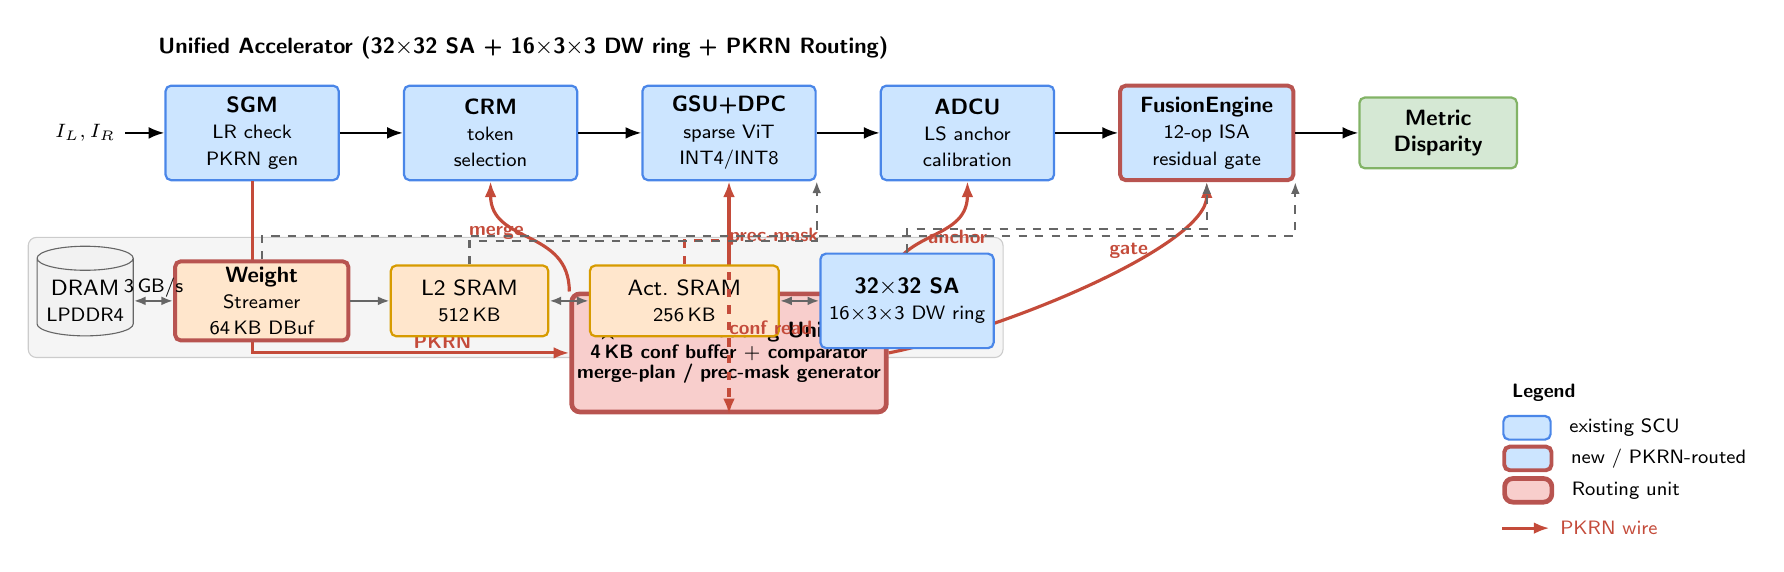
\begin{tikzpicture}[
  font=\footnotesize\sffamily,
  node distance=3mm,
  stage/.style={draw=calcStroke, fill=calcFill, rounded corners=2pt, thick,
                minimum width=22mm, minimum height=12mm, align=center, inner sep=2pt},
  newstage/.style={draw=newStroke, fill=calcFill, rounded corners=2pt, line width=0.5mm,
                   minimum width=22mm, minimum height=12mm, align=center, inner sep=2pt},
  mem/.style={draw=memStroke, fill=memFill, rounded corners=2pt, thick,
              minimum width=20mm, minimum height=9mm, align=center, inner sep=2pt},
  newmem/.style={draw=newStroke, fill=memFill, rounded corners=2pt, line width=0.5mm,
                 minimum width=22mm, minimum height=9mm, align=center, inner sep=2pt},
  dram/.style={draw=dramStroke, fill=dramFill, cylinder, shape border rotate=90,
               aspect=0.25, minimum height=9mm, minimum width=12mm, align=center},
  outp/.style={draw=dataStroke, fill=dataFill, rounded corners=2pt, thick,
               minimum width=20mm, minimum height=9mm, align=center, inner sep=2pt,
               font=\footnotesize\sffamily\bfseries},
  pruBox/.style={draw=hubStroke, fill=hubFill, rounded corners=3pt, line width=0.6mm,
                 minimum width=36mm, minimum height=15mm, align=center, inner sep=2pt,
                 font=\footnotesize\sffamily\bfseries},
  arr/.style={-{Latex[length=2mm]}, thick},
  pkrnarr/.style={-{Latex[length=2mm]}, draw=pkrnCol, line width=0.4mm},
  pkrndash/.style={-{Latex[length=2mm]}, draw=pkrnCol, line width=0.35mm, dashed},
  membus/.style={-{Latex[length=1.5mm]}, thick, draw=dramStroke},
  lbl/.style={font=\scriptsize\sffamily, inner sep=1pt},
  plbl/.style={font=\scriptsize\sffamily\bfseries, text=pkrnCol, inner sep=1pt}
]

% ============= TOP ROW: 5-STAGE LTR PIPELINE =============
\node[stage] (sgm) at (0,0) {\textbf{SGM}\\\scriptsize LR check\\\scriptsize PKRN gen};
\node[stage, right=8mm of sgm] (crm)  {\textbf{CRM}\\\scriptsize token\\\scriptsize selection};
\node[stage, right=8mm of crm] (gsu)  {\textbf{GSU+DPC}\\\scriptsize sparse ViT\\\scriptsize INT4/INT8};
\node[stage, right=8mm of gsu] (adcu) {\textbf{ADCU}\\\scriptsize LS anchor\\\scriptsize calibration};
\node[newstage, right=8mm of adcu] (fe) {\textbf{FusionEngine}\\\scriptsize 12-op ISA\\\scriptsize residual gate};

% outputs
\node[outp, right=8mm of fe] (disp) {Metric\\Disparity};

% data path
\draw[arr] (sgm) -- (crm);
\draw[arr] (crm) -- (gsu);
\draw[arr] (gsu) -- (adcu);
\draw[arr] (adcu) -- (fe);
\draw[arr] (fe) -- (disp);

% input
\node[left=5mm of sgm, font=\scriptsize\sffamily] (inp) {$I_L,I_R$};
\draw[arr] (inp) -- (sgm);

% ============= PKRN ROUTING UNIT (above SRAM read path, fans out to 4 units) =============
\node[pruBox, below=14mm of gsu] (pru) {%
  $\bigstar$ PKRN Routing Unit $\bigstar$\\[-2pt]
  \scriptsize 4\,KB conf buffer $+$ comparator\\[-2pt]
  \scriptsize merge-plan / prec-mask generator
};

% PKRN intake from SGM into PRU
\draw[pkrnarr] (sgm.south) |- (pru.west) node[pos=0.8, above, plbl] {PKRN};

% Fan-out: PRU emits merge-plan, prec-mask, anchor-idx, gate-map
\draw[pkrnarr] (pru.north west) .. controls +(0,8mm) and +(0,-8mm) .. (crm.south)
  node[pos=0.55, plbl, left=-0.5mm] {merge};
\draw[pkrnarr] (pru.north) -- (gsu.south)
  node[pos=0.5, plbl, right=-0.5mm] {prec-mask};
\draw[pkrnarr] (pru.north east) .. controls +(0,8mm) and +(0,-8mm) .. (adcu.south)
  node[pos=0.5, plbl, right=-0.5mm] {anchor};
\draw[pkrnarr] (pru.east) .. controls +(15mm,3mm) and +(0,-8mm) .. (fe.south)
  node[pos=0.6, plbl, above] {gate};

% ============= MEMORY SUBSYSTEM (bottom, backs all stages) =============
\node[dram, below=12mm of inp] (dram) {DRAM\\\scriptsize LPDDR4};
\node[newmem, right=5mm of dram] (ws) {\textbf{Weight}\\\scriptsize Streamer\\\scriptsize 64\,KB DBuf};
\node[mem, right=5mm of ws] (l2) {L2 SRAM\\\scriptsize 512\,KB};
\node[mem, right=5mm of l2, minimum width=24mm] (actsr) {Act.\ SRAM\\\scriptsize 256\,KB};
\node[stage, right=5mm of actsr, minimum width=22mm] (sa) {\textbf{32$\times$32 SA}\\\scriptsize 16$\times$3$\times$3 DW ring};

\begin{pgfonlayer}{background}
  \node[fit=(dram)(sa), fill=gray!8, rounded corners=3pt, inner sep=3pt, draw=gray!40] (membox) {};
\end{pgfonlayer}

% memory buses
\draw[membus, {Latex[length=1.5mm]}-{Latex[length=1.5mm]}] (dram.east) -- node[lbl, above]{3\,GB/s} (ws.west);
\draw[membus] (ws.east) -- (l2.west);
\draw[membus, {Latex[length=1.5mm]}-{Latex[length=1.5mm]}] (l2.east) -- (actsr.west);
\draw[membus, {Latex[length=1.5mm]}-{Latex[length=1.5mm]}] (actsr.east) -- (sa.west);

% act-sram read path feeds PRU (this is the key routing: PRU reads conf off the activation SRAM)
\draw[pkrnarr, dashed] (actsr.north) -- ++(0,3mm) -| (pru.south)
  node[pos=0.75, plbl, right=-0.5mm] {conf read};

% memory-to-stage bus arrows (dashed)
\draw[membus, dashed] (ws.north) -- ++(0,3mm) -| (fe.south east);
\draw[membus, dashed] (l2.north) -- ++(0,3mm) -| (gsu.south east);
\draw[membus, dashed] (sa.north) -- ++(0,3mm) -| (fe.south);

% ============= LABEL / TITLE =============
\node[font=\footnotesize\sffamily\bfseries, anchor=south west]
  at ($(sgm.north west)+(-2mm,2mm)$) {Unified Accelerator (32$\times$32 SA + 16$\times$3$\times$3 DW ring + PKRN Routing)};

% ============= LEGEND =============
\begin{scope}[shift={($(disp.south east)+(-2mm,-26mm)$)}]
  \node[anchor=north west, font=\scriptsize\sffamily\bfseries] (lh) at (0,0) {Legend};
  \node[stage, minimum width=6mm, minimum height=3mm, below=0.5mm of lh.south west, anchor=north west, inner sep=1pt] (l1) {};
  \node[right=1mm of l1, font=\scriptsize\sffamily] {existing SCU};
  \node[newstage, minimum width=6mm, minimum height=3mm, below=0.5mm of l1.south west, anchor=north west, inner sep=1pt] (l2) {};
  \node[right=1mm of l2, font=\scriptsize\sffamily] {new / PKRN-routed};
  \node[pruBox, minimum width=6mm, minimum height=3mm, below=0.5mm of l2.south west, anchor=north west, inner sep=1pt, font=\scriptsize] (l3) {};
  \node[right=1mm of l3, font=\scriptsize\sffamily] {Routing unit};
  \draw[pkrnarr] ([yshift=-3mm]l3.south west) -- ++(6mm,0)
    node[right, font=\scriptsize\sffamily, text=pkrnCol] {PKRN wire};
\end{scope}

\end{tikzpicture}
\end{document}
